    \subsection{Recovery of the Schwarzschild Metric}
      \label{subsec:recovery-of-the-schwarzschild-metric}

      For a static, spherically symmetric distribution of particle excitations, the $\chi$ field satisfies
      \begin{equation}
        \nabla^2 \chi(r) \propto \rho(r).
      \end{equation}

      Solving this equation in the weak-field limit yields an effective metric equivalent to the Schwarzschild solution
      of general relativity:
      \begin{equation}
        ds^2 = -\left(1 - \frac{2GM}{r}\right)c^2 dt^2 + \left(1 - \frac{2GM}{r}\right)^{-1} dr^2 + r^2 d\Omega^2 ,
      \end{equation}
      with the gravitational constant $G$ emerging as a derived quantity determined by the coupling between $\chi$
      and particle excitations.

      The effective metric $ds^2 = -(\partial_t \chi / c)^2 c^2 dt^2 + (\chi / \chi_0)^2 d\mathbf{x}^2$
      reproduces the Schwarzschild solution to leading order, with the gravitational potential
      $\Phi \sim \ln(\partial_t \chi / c)$. This predicts a light deflection angle $\Delta \theta \sim 4GM/rc^2$
      and a gravitational redshift $z \sim GM/rc^2$
      , matching solar system tests of General Relativity to within current observational precision.

      \begin{figure}[htbp]
        \centering
        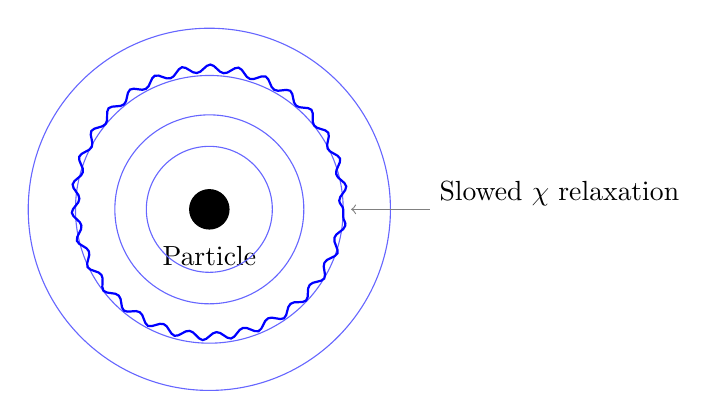
\begin{tikzpicture}[scale=1]

% Central mass
          \filldraw[black] (0,0) circle (0.25);
          \node[below] at (0,-0.35) {Particle};

% Phase lines
          \foreach \r in {0.8,1.2,1.7,2.3} {
            \draw[blue!60] (0,0) circle (\r);
          }

% Distortion
          \draw[blue, thick, decorate, decoration={snake, amplitude=0.5mm}]
          (0,0) circle (1.7);

% Arrows
          \draw[->, gray] (2.8,0) -- (1.8,0);
          \node[right] at (2.8,0.2) {Slowed $\chi$ relaxation};

        \end{tikzpicture}
        \caption
        {Emergence of gravity in Cosmochrony. Localized excitations of $\chi$ slow down the relaxation rate of the field
          ,inducing differential proper-time flow and an effective metric curvature analogous to gravitational time
        dilation.}
        \label{fig:chi_gravity}
      \end{figure}

      \textit{On the Necessity of the Metric Form:
      The use of an effective metric to describe the coupling between the field and local trajectories is not an
      arbitrary ansatz, but the minimal geometric representation of the field's influence.
      As demonstrated in our framework, the induced metric structure
        (of the form $g_{\mu\nu} \propto \partial_\mu \chi \partial_\nu \chi$ or its perturbations) is fundamentally
        linked to the field’s self-coupling and the solitonic scale. While the Einstein-Hilbert action is not derived
        here from first principles, it is recovered as the leading-order effective description of the $\chi$-gradients
        in the long-wavelength limit. Schwarzschild-like solutions thus emerge by necessity from the requirement that
        the field remains in a state of local equilibrium (minimal relaxation) around localized solitons.}
